\let\negmedspace\undefined
\let\negthickspace\undefined
\documentclass[journal]{IEEEtran}
\usepackage[a5paper, margin=10mm, onecolumn]{geometry}
%\usepackage{lmodern} % Ensure lmodern is loaded for pdflatex
\usepackage{tfrupee} % Include tfrupee package

\setlength{\headheight}{1cm} % Set the height of the header box
\setlength{\headsep}{0mm}     % Set the distance between the header box and the top of the text

\usepackage{gvv-book}
\usepackage{gvv}
\usepackage{cite}
\usepackage{amsmath,amssymb,amsfonts,amsthm}
\usepackage{algorithmic}
\usepackage{graphicx}
\usepackage{textcomp}
\usepackage{xcolor}
\usepackage{txfonts}
\usepackage{listings}
\usepackage{enumitem}
\usepackage{mathtools}
\usepackage{gensymb}
\usepackage{comment}
\usepackage[breaklinks=true]{hyperref}
\usepackage{tkz-euclide} 
\usepackage{listings}
% \usepackage{gvv}                                        
\def\inputGnumericTable{}                                 
\usepackage[latin1]{inputenc}                                
\usepackage{color}                                            
\usepackage{array}                                            
\usepackage{longtable}                                       
\usepackage{calc}                                             
\usepackage{multirow}                                         
\usepackage{hhline}                                           
\usepackage{ifthen}                                           
\usepackage{lscape}
\usepackage{circuitikz}
\tikzstyle{block} = [rectangle, draw, fill=blue!20, 
    text width=4em, text centered, rounded corners, minimum height=3em]
\tikzstyle{sum} = [draw, fill=blue!10, circle, minimum size=1cm, node distance=1.5cm]
\tikzstyle{input} = [coordinate]
\tikzstyle{output} = [coordinate]


\begin{document}

\bibliographystyle{IEEEtran}
\vspace{3cm}

\title{8-8.3-3}
\author{EE24BTECH11064 - Harshil Rathan}
 \maketitle
% \newpage
% \bigskip
{\let\newpage\relax\maketitle}

\renewcommand{\thefigure}{\theenumi}
\renewcommand{\thetable}{\theenumi}
\setlength{\intextsep}{10pt} % Space between text and floats


\numberwithin{equation}{enumi}
\numberwithin{figure}{enumi}
\renewcommand{\thetable}{\theenumi}

\textbf{Question}:\\
Find the area of the region lying in the first quadrant and bounded by $y=4x^2$, $x=0$, $y=1$ and $y=4$. \\ 
\solution \\
THe equation of the curve is 
\begin{align}
     y = 4x^2
     \label{0.1}
\end{align}
\begin{align}
    x = \frac{\sqrt{y}}{2}
\end{align}
w.k.t that \ref{0.1} is an upward parabola symmetric about y-axis\\
\textbf{Theory}
\begin{align}
    \int_1^4 x \, dx = \int_1^4 \left| \frac{\sqrt{y}}{2} \right| dy
\end{align}
\begin{align}
    \frac{1}{2} \int_1^4 y^{\frac{1}{2}} \, dy = \frac{1}{2} \left| \frac{y^{\frac{3}{2}}}{\frac{3}{2}} \right|_1^4
\end{align}
\begin{align}
    = \frac{1}{2} \cdot \frac{2}{3} \left[ 4^{\frac{3}{2}} - 1^{\frac{3}{2}} \right]
\end{align}
\begin{align}
    = \frac{1}{3} \left( 4\sqrt{4} - 1 \right) = \frac{1}{3} (8 - 1) = \frac{7}{3} \ = 2.3333 \text{ sq. units.} 
\end{align}
\textbf{Solution using Trapezoidal Rule}\\
Divide the interval [1,4], into n = 1000 sub intervals\\
The step size is:
\begin{align}
    h=\frac{4-1}{1000} = 0.003
\end{align}
The y-values at sub interval points are
\begin{align}
     y_i = 1 + i\cdot h \text{  for i = 1,2,3$\cdots$ ,1000}
 \end{align}
\begin{align}
     y_0 = 1 \text{,  } y_1 = 1.003 \text{, }y_2 = 1.006 \text{, } \cdots ,y_{1000} = 4 
\end{align}
Compute the corresponding $x_i$ values 
\begin{align}
    x_i = \frac{\sqrt{y_i}}{2}
\end{align}
\begin{align}
     x_0 = \sqrt{\frac{1}{4}} = 0.5 \text{, }x_1 = \sqrt{\frac{1.003}{4}} \text{, }x_2 = \sqrt{\frac{1.006}{4}}\cdots, x_{1000}= 1
\end{align}
Apply Trapezoidal rule 
\begin{align}
    Area \approx \frac{h}{2} \left[ x_0 + 2(x_1 + x_2 + \dots + x_{n-1}) + x_n \right].
\end{align}
General difference equation \\
Substitute \( y_i = 1 + i h \) into \( x_i \)
\begin{align}
    x_i = \sqrt{\frac{1 + i h}{4}}
\end{align}
\begin{align}
   x_i = \sqrt{\frac{1 + \frac{3i}{n}}{4}}, \quad i = 0, 1, 2, \ldots, n.
\end{align}
\begin{align}
    A \approx \frac{h}{2} \left[ \sqrt{\frac{1}{4}} + 2 \sum_{i=1}^{n-1} \sqrt{\frac{1 + \frac{3i}{n}}{4}} + \sqrt{\frac{4}{4}} \right]
\end{align}
\begin{align}
    A \approx \frac{3}{2n} \left[ \frac{1}{2} + 2 \sum_{i=1}^{n-1} \sqrt{\frac{1 + \frac{3i}{n}}{4}} + 1 \right]
    \label{0.16}
\end{align}
Substituting n = 1000 in \ref{0.16}
\begin{align}
    A \approx \frac{0.003}{2} \left[ \frac{1}{2} + 2 \sum_{i=1}^{999} \sqrt{\frac{1 + 0.003i}{4}} + 1 \right]
    \label{0.17}
\end{align}
On simplying \ref{0.17} we get 
\begin{align*}
    \text{Area = 2.3333}
\end{align*}
The solution is hence verified with the theoretical solution 
\begin{figure}
    \centering
    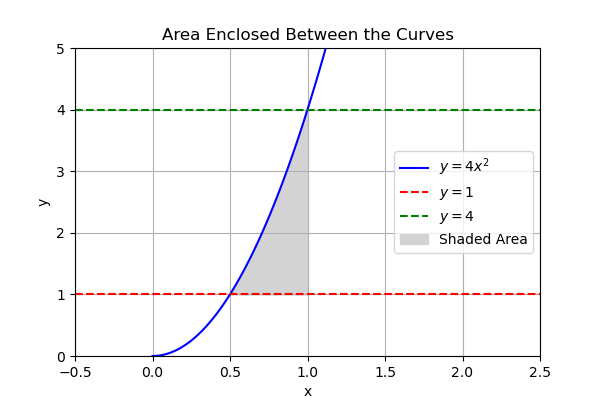
\includegraphics[width=\columnwidth]{figs/Figure_1.png}
\end{figure}
\end{document}



